The WR protocol requires a network topology similar to the ITU-T G.8275.1/Y.1369.1 standard, a IEEE-1588v2 telecommunication profile that describes a time-aware network capable to provide full timing support \cite{itu:TG8275_1_Y_1369_1} as explained in previous section. It uses a master time reference (SKA1 clock) that is distributed following a tree topology in a master-slave configuration. The SKA PPS distribution system is composed of two different kinds of devices: 

\begin{itemize}
	\item {The WR Switches \cite{sevensols:wr_switch}. They are standard 1U height rack-mounted equipment with 18 SFP ports and are placed in the CSPs at each of the clock ensembles. For SKA1-MID, one is placed halfway along each of the 3 spiral arms to regenerate the signal for the longest links.}
	\item{The end-nodes. They consist of a WR-ZEN node \cite{sevensols:wr_zen} powered by a Zynq FPGA-SoC and placed on inside a 1U rack enclosure. They will be located at the cores of SKA1-LOW and SKA1-SURVEY, along their spiral arms, one for each SKA1-MID dish and one for each CSP.}
\end{itemize}

The WR switches are responsible for generating the WR timing signal from the SAT clock ensembles. They lock to an external 10MHz reference and to a PPS signal, and use NTP or IRIG-B to determine the UTC time of each PPS edge. Synchronization between WR devices is performed over a a single fiber link up to 120 km using commercial SFPs.
However, the distances for SKA1-MID are longer and it is necessary to use 
intermediate WR switches as repeaters with a penalty over the system 
performance due to increment of the inherent noise of each WR device that it is 
propagated to the down-link nodes. An analysis of the jitter evolution for 
network with many hops could be read in \cite{torres2016scalability}. Thanks to 
network similarities between WR and SKA, both can use the same single fiber 
strand available for the SAT network. 

\begin{figure}[H]
	\centering
	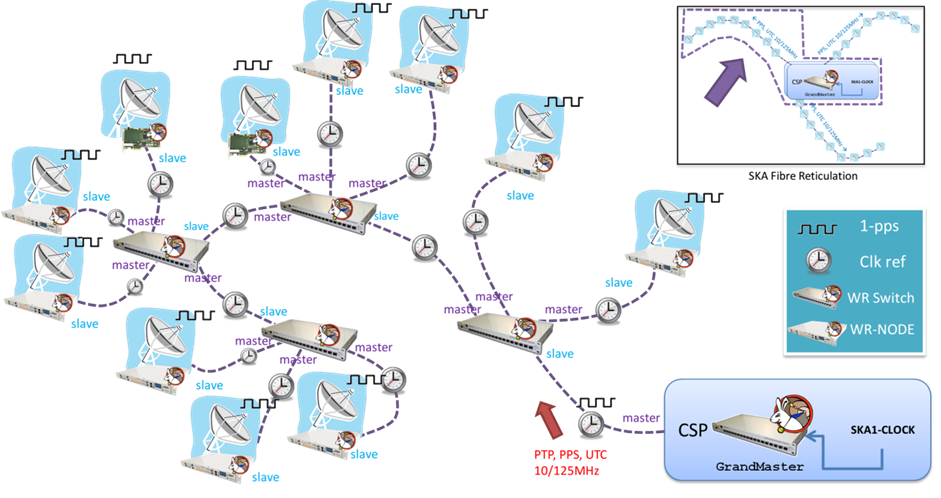
\includegraphics[scale=0.4]{img/ska_pps_network}
	\caption{Network topology for PPS signal distribution based on WR switches and nodes. The figure shows the different elements and the network topology. }
	\label{fig:ska_pps_dist_network}
\end{figure}

An important feature of the system to take into account is that the PPS pulse itself at each station is derived from the reference frequency distributed from the SKA clock and not from the WR system. In normal operations, the WR system only monitors the absolute time of each PPS and reports it back activating an alert if the PPS signal does not align with the start of the UTC second. This condition indicates something is wrong in the timing chain and the station must be discard data to ensure not to introduce corrupt one in the system. Other functionality associated with the WR part is to temporarily alter the division ratio to bring the PPS edge back in alignment with UTC time. In this case, fringe finding must then be performed to restore full calibration again.

The centrally located WR switches and the WR end-nodes are connected to by a 
single strand of single-mode fiber with LC/PC connectors and industry standard 
bi-directional SFPs that use two wavelengths (down-link and up-link) to produce 
optical signals to be transmitted. Finally the end nodes generate a 1PPS signal available. 

As previously described, this solution requires WR switches and nodes. The former are well-defined equipment with known interfaces and software support. 

For the implementation of the SKA nodes, we have proposed the utilization of the WR-ZEN board. Thanks to this new platform, the utilization of a host computer/crate to host the FPGA card can be avoided which reduces significantly the equipment price and is also a remarkable improvement in term of dependability which is a key factor taking into account that SKA Telescope should have an annual availability of about 95\% of the time (although degraded operation modes can be allowed under some circumstances).
Finally note that all these features are possible keeping the full flexibility of a complete CPU+FPGA system on a single board. 

In the following section we will describe the proposed node hardware, gateware and firmware that have been developed as a candidate solution for the SKA Telescope PPS distribution system. 

\subsection{A PPS distribution node architecture} \label{subsec:ska-pps-system-arch}

The PPS distribution system for SKA is based on the WR-ZEN platform that provides the WR support in order to ensure the synchronization accuracy in the system. The first design of the PPS system includes the Fine Delay FMC card that is used to generate the timing signals through mezzanine channels and has two Network Interface Cores (NIC) that allows accessing optical fiber ports as conventional Linux network interfaces. An introduction to this platform is presented in \cite{migueljl-paper-wr-zen-intro} and a contribution that improves the NIC bandwidth of the design in \cite{jorgesg-paper-wr-zen-dma}. Moreover, the WR-ZEN is also under study for other FMC cards such as the FMC ADC one to build a distributed oscilloscope \cite{joselj-paper-wr-zen-adc}.

Nowadays, the utilization of the Fine Delay FMC card is still under discussion and there is a possible design whose its final architecture could be addressed without this module.

\subsubsection{Hardware}
\label{subsec:hardware}

The WR-ZEN board is a proprietary design of the Seven Solutions company 
developed in 2015. The major design changes respect to previous designs for 
WR-nodes are the inclusion of a Zynq FPGA-SoC platform from Xilinx, and a 
flexible clocking scheme. The former, enables a more structured design where 
the software can be organized in abstraction layers. This is achieved by the 
inclusion of an Linux-like OS and many low-level drivers and a Hardware 
Abstraction Layer (HAL) whose most important result is an easy and quick 
development of new functionalities on top of all the software that interfaces 
with the underlying hardware. A deeper detailing of the software structure is 
given at subsection \ref{subsec:software}. The latter, makes the new board 
suitable for many synchronization applications with diverse requirements.

\begin{figure}[H]
	\centering
	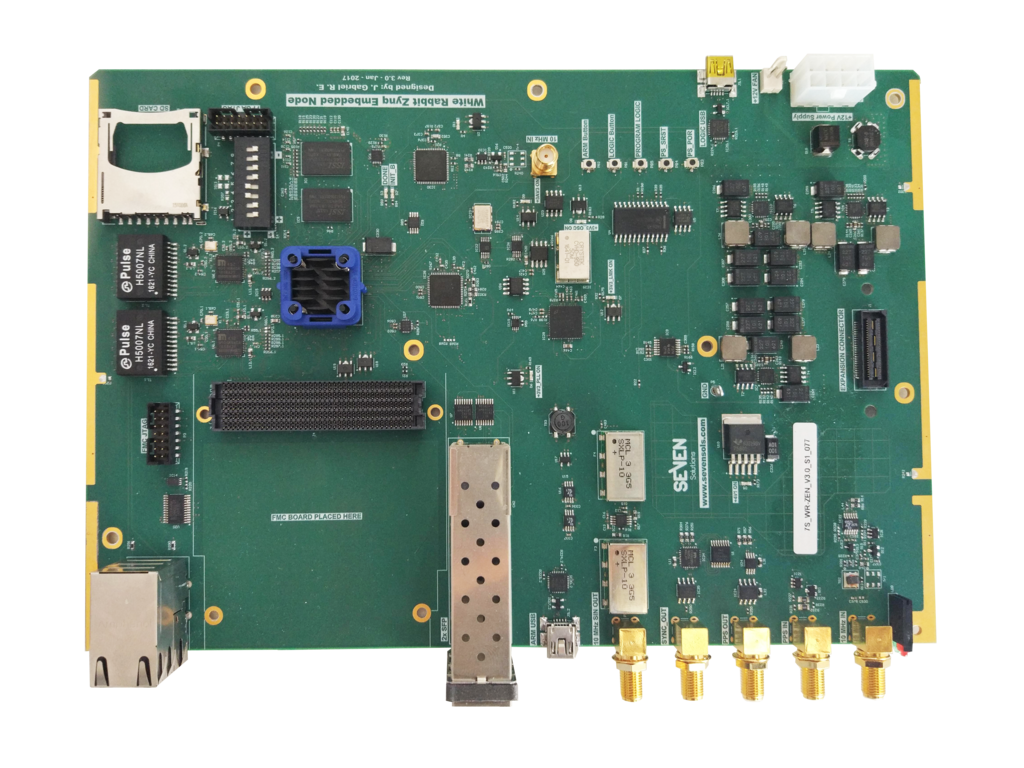
\includegraphics[width=0.7\linewidth]{img/wrzenv3_scaled}
	\caption[WR-ZEN board picture]{The picture shows the WR-ZEN board with the 
	FMC Fine Delay connected. Main connectors are shown: Ethernet ports, SFP 
	ports and the SMA connectors for the RF input/output signals.}
	\label{fig:wrzen}
\end{figure}

The FPGA-SoC platform breaks up design in two different parts: (i) the 
Programmable Logic (PL) including modules described in HDL; and (ii) the 
Processing System (PS) formed by all the software executed by the ARM processor.
The inclusion of a hard-processor is something new in the node architecture.
These problems have been solved by the WR-ZEN design: a 
powerful hard-processor for software and more free resources in the FPGA side 
due to pass some of the software from the embedded-processor to the ARM. In 
addition to that, the Zynq platform includes the needed physical components by 
the WR design: internal programmable PLLs, Gigabit Transceiver Ports (GTPs), 
and other not strictly fundamental por a WR-node but which could be very 
helpful in future designs such as Ethernet interfaces with hw timestamping 
support (allowing PTPv2 support). I/O ports are also very important because 
they will interface with external components which can obtain synchronization 
from the base board. The most relevant I/O interfaces of the WR-ZEN are the FMC 
HPC socket (support for the OHWR \cite{ohwr:repo} FMC cards 
\cite{ohwr:fmc-fine-delay}), two SFPs sockets capable of BC configurations, and 
many external RF connectors for input/output of RF signals and the PPS.

\begin{figure}
	\centering
	\includegraphics[width=0.7\linewidth]{img/zenclkschema}
	\caption[WR-ZEN clocking schema]{The figure depicts the new clocking schema 
		presented in the WR-ZEN desing. The most relevant changes considering 
		previous designs are: the inclusion of an external PLL to lock an 
		external 
		stable clock reference (GrandMaster mode), and a flexible path in the 
		main 
		clocks path allowing the final user to choose between a low-noise PLL 
		and a 
		full-featured PLL with many options such as programmable output delays.}
	\label{fig:zenclkschema}
\end{figure}

The extended WR clock schema is depicted in Figure \ref{fig:zenclkschema}. 
Besides including new components, the WR-ZEN design, upgrades some of them 
looking for an increment of the clock stability. All the clock path: DAC, VCXO, 
PLL has received an upgrade. A new DAC with a better response time and 
stability, and low-noise VCXO and PLL have been included. But the PLL from 
previous designs is maintained because it offers some key aspects such as 
programmable output delays. To avoid cascading many PLLs, the signal from the 
XO is droved to the low-noise PLL first because it allows bypassing its 
reference to other components without adding noise to the reference. This 
schema enables using both PLLs at the same time. One of them is used to 
generate all the WR-clocks and the other could be used to generate custom 
frequencies not available from the other for example. The WR general 
performance is limited by the noise when locking to an external reference, in 
the so called GranMaster mode, described in \cite{Rizzi2016}. The conclusion of 
that contribution is that in order to decrease the noise when locking to an 
external reference, internal PLLs in the FPGA should be avoid. Instead of it, 
it is recommended an Analog external PLL which locks to the external reference 
and generated the needed clock signal by the internal elements of the WR-logic 
in the FPGA. That results are included in the version 3.0 of the WR-ZEN as 
shown in Figure \ref{fig:zenclkschema} looking to achieve the expected PPS 
distribution stability requirements of the SKA project.


\subsubsection{Gateware}
\label{subsec:gateware}

The gateware (FPGA firmware) is responsible for configuring the embedded ARM microprocessor and the FPGA inside the Zynq SoC. The main block diagram is shown in the Fig. \ref{fig:gateware_first_level}. It includes the WRPC Dual port core that implements the high accuracy timing protocol based on White Rabbit and provides basic capabilities such as Gigabit networking, timestamp mechanism, debug interfaces, etc. The GT ports include the Gitabit transceiver needed to send/receive packets to/from the network. The NIC cores are in charge of processing the incoming/outcoming packets and notify these events to the ARM. The TxTSU is an additional module that allows recovering the outcoming packet timestamps. The Fine Delay core controls the operation of the Fine Delay FMC card if any is plugged into the FMC socket. The WB Crossbar interconnects all the elements of the architecture and eases the configuration process performed by the ARM. The AXI-WB Bridge is a bus converter between AMBA AXI and Wishbone ones. This conversion is needed because the ARM microprocessor uses the AMBA specification while others components are based on WB.

\begin{figure}[H]
	\centering
	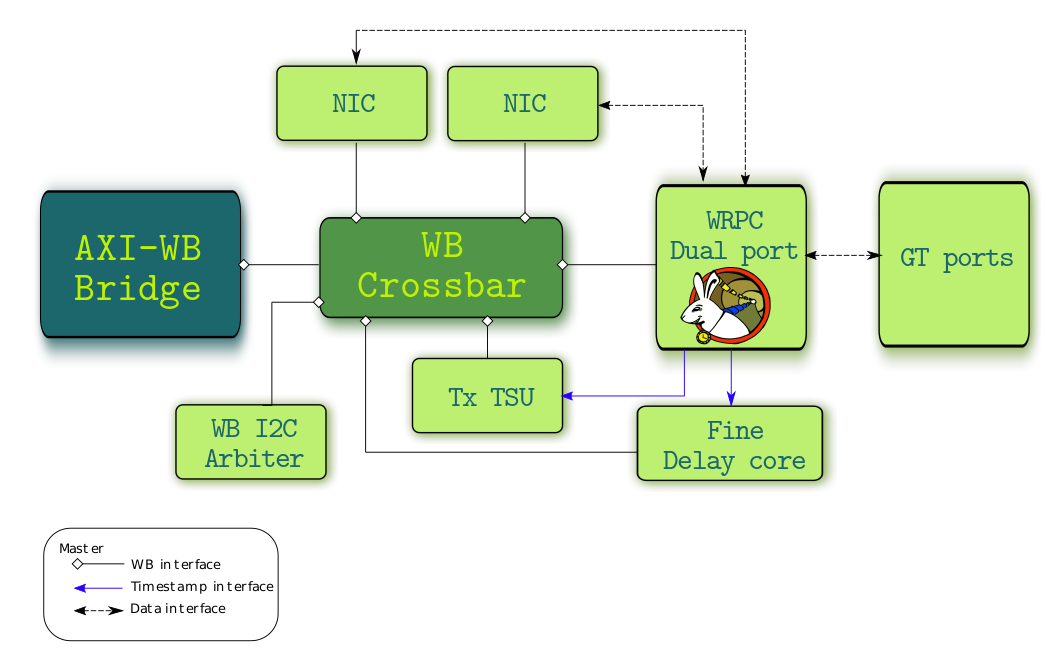
\includegraphics[scale=0.4]{img/gateware_first_level}
	\caption{Gateware project design. The figure shows the main components of the design. The most important one is the WRPC dual port that is responsible for implementing the WR protocol. The Gigabit Transceiver ports allows to transmit/receive packets to/from the network through the optical SFP modules. The NIC cores manage Ethernet packets and behave as standard network interface cards for the ARM microprocessor. The AXI-WB Bridge translates AXI transactions into WB ones. It is important because the ARM is connected using AMBA specification meanwhile the WR FPGA cores use Wishbone bus standard. Finally, the Fine Delay core contains the resources needed to control the Fine Delay FMC card.}
	\label{fig:gateware_first_level}
\end{figure}

\subsubsection{Firmware} \label{subsec:firmware}

The firmware code is related to all the functionalities needed by the WR protocol. In the node architecture, the embedded software part of the WR 
protocol and some device drivers runs in the soft-microprocessor describe in 
the previous section. The main tasks of the WR routines are the servo 
loop algorithm which, maintains the lock to the recovered frequency from the 
master device, and the implementation of the WR-PTP stack. In addition, a 
simple Command Language Interface (CLI) is introduced to allow 
the user interaction when it is used in standalone mode without an external PC.

\subsubsection{Software} \label{subsec:software}

The WR-ZEN is the first WR node taking advantage of a Linux 
based operative system (OS). Due to the inclusion of a dual-core ARM 
microprocessor in the platform, the system design is not longer tied to 
low-level software design. New functionalities, such as communication 
protocols, management tools, etc., are quickly added thanks to the support 
provided by the OS: a hardware abstraction layer, and drivers which abstract 
the management of the underlaying logic. This middleware adds also more 
security controlling the access to the hardware.

The software components are presented in the Fig. \ref{fig:software_architecture}.
It is divided into the userspace utilities and the kernel support. 
The former include the Zen library that implements the basic functionalities for the Zen tools through the C standard library. The Zen tools provides some mechanisms to program the FPGA
design and connect to the internal UART for debugging/configuration tasks among others. 
Moreover, other utilities are included to control the Fine Delay FMC card if it is plugged into the FMC socket.

In the kernel side, some kernel drivers have been implemented. The main one is the \textit{zen}
driver that is responsible for setting up all the IP cores in the FPGA and creates the 
standard Linux network interfaces. The \textit{fmc} and \textit{zio} drivers are retrieved from the 
OHWR repository and implements a generic support for FMC and ZIO buses respectively. 
The \textit{zio} driver has been modified in order to work properly in the WR-ZEN platform.
The \textit{zen-nic} kernel modue is in charge of enabling/desabling the network capabilities of 
the zen driver. The \textit{fmc-fine-del} driver provides basic functionalities for the Fine Delay FMC card.

As previously mentioned, there are dependencies between the different kernel drivers and it establishes the installation order. The \textit{zen} one depends on \textit{fmc}. The \textit{fmc-fine-del} needs \textit{zen}, \textit{zio} and \textit{fmc}. The \textit{zen-nic} only uses the \textit{zen}.

\begin{figure}[H]
	\centering
	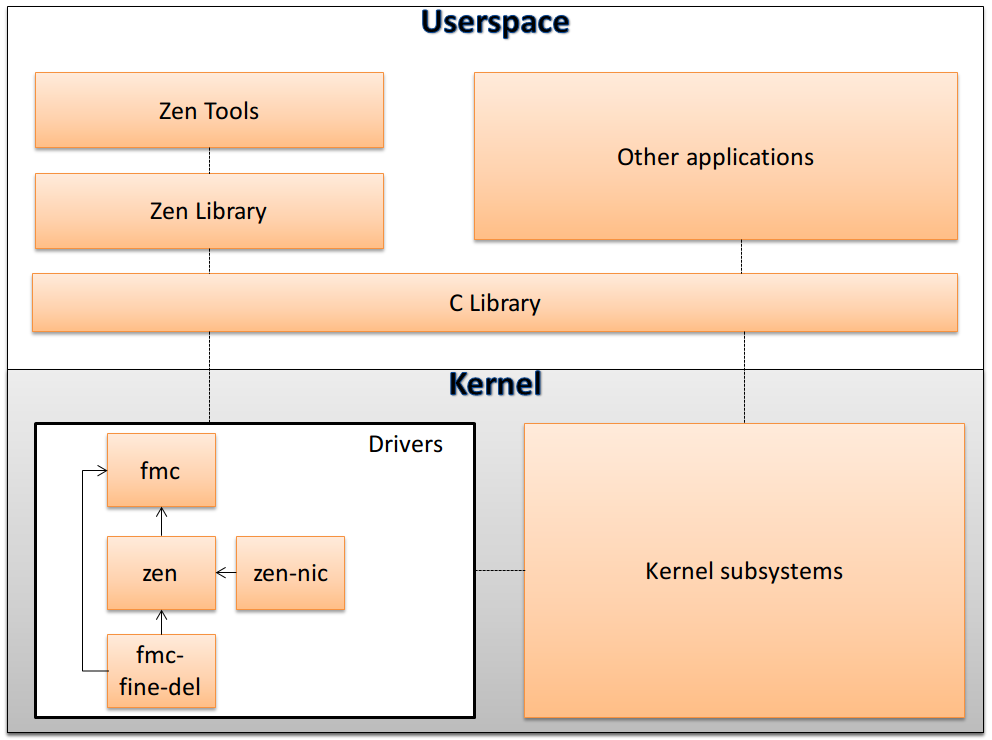
\includegraphics[scale=0.4]{img/software_architecture}
	\caption{Software architecture. The picture shows the software architecture
		used by the design. It is based on Linux kernel and several tools and drivers
		have been developed for the WR-ZEN board. The tools can be used to program 
		the FPGA, update the soft-microprocessor code or connect to the virtual UART
		interface of the WRPC-2p. They call the Zen Library procedures that finally
		use C Library functions and switch to kernel mode through system calls. In the
		kernel space, the drivers are responsible for implementing all the requested 
		functionalities. }
	\label{fig:software_architecture}
\end{figure}

The next section describes the main experiments performed and the results obtained.

